\scanpage{111}

\[
\Sigma_J=\mathbb{P}(W(J))\simeq\check{\mathbb{P}}(V(J))
\]
\diagram{\begin{tikzcd}[ampersand replacement=\&]
\unsure{\cdot|0} \arrow[r,dash] \& V(J) \arrow[r] \& \mathcal{O}^J \arrow[r,"\text{somme}"'] \& \mathcal{O} \arrow[r] \& 0
\end{tikzcd}}

\deleted{suite}
\diagram{\begin{tikzcd}[ampersand replacement=\&]
0 \arrow[r] \& F \arrow[r] \& V(J)_\Sigma \arrow[r] \& \mathcal{O}_\Sigma(1) \arrow[r,dash] \& 0
\end{tikzcd}}

\[
F(1)\simeq\mathcal{O}(\omega)
\qquad
(\mathcal{O}\ \text{tordu par }\underline{\omega}=\underline{\omega}(J)\unsure{\,\},}\ \text{i.e. }\det V(J))
\]
\inserted{et}
\[
\mathcal{O}(1)\simeq\check{F}(\omega)
\qquad
\left(\text{par }F\wedge\mathcal{O}_\Sigma(1)
\mathrel{\mathop{\simeq\!\longrightarrow}\limits_{\text{prod. ext.}}}
\det V(J)_\Sigma\simeq\mathcal{O}_\Sigma(\omega)\deleted{\unsure{\Sigma}}\right)
\]
\margin{attention signes!}

\margin{%
$F\times V(J)\longrightarrow\underline{\mathcal{O}}$

Accouplement donné (\deleted{\unsure{fixant|défini par}} un ordre circulaire \unsure{fixé} \deleted{\unsure{en prenant}} $(i,j,k)$), par
$x\wedge y\wedge e_i=x\wedge y\wedge e_j=x\wedge y\wedge e_k$
où $x\in F$, $y\in V(J)$ \unsure{mod} $F$
i.e. donné par \unsure{les mineurs|les 2 mineurs} de la matrice de $(x,y)$.
}

\[
\Omega^1_\Sigma\deleted{\unsure{0}}\simeq F(-1)\simeq\mathcal{O}(\unsure{-2})(\underline{\omega})
\]
\[
\check{\Omega}^1_\Sigma\simeq\mathcal{O}(2)(\underline{\omega})
\qquad\text{fibré tangent à }\Sigma
\]

\margin{$\deleted{\unsure{\varphi_{ij}+\varphi_{jk}+\varphi_{ki}=0}}$}

Points $R_i$ \inserted{\figure{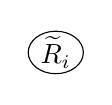
\begin{tikzpicture}[baseline=(r.base)]\node (r) at (0,0) {$\widetilde{R}_i$};\draw (0,0) ellipse (0.35 and 0.27);\end{tikzpicture}}} $(i\in J)$ (``trous'') de $\Sigma$ et $P\Sigma$

\[
\begin{gathered}
R_i\subset\unsure{V|W}(J)\\
\Vert\\
\mathcal{O}_{\unsure{\Sigma}}(e_k-e_j)\\
\simeq\mathcal{O}(\underline{\omega})
\end{gathered}
\qquad\mathcal{O}(1)_{R_i}\simeq\mathcal{O}
\]
\unsure{en associant} à $e_k-e_j$ l'orientation $(i,j,k)$

\margin{%
$\widetilde{R}_i$ pt au-dessus de $R_i$
image de $e_i-e_j=\varphi_{ji}$
$(\equiv e_i-e_k)$ dans $V(J)/R_i$
}

\deleted{Points \unsure{les} $\widetilde{R}_i$ de $P\Sigma_J=\check{V}^{*}(\mathcal{O}_\Sigma(1))$ l'élément $1$ au-dessus de $R_i$.}

\[
\Gamma(\Sigma_{\deleted{\unsure{J}}},\mathcal{O}_\Sigma(1))\simeq V(J)
\]
\deleted{$e_j-e_k$ section $\unsure{\omega_{j,k}}$}
\[
\varphi_{jk}=e_k-e_j\in\Gamma(\Sigma,\mathcal{O}_\Sigma(1))
\]
nulle en $R_i$
\[
\varphi_{kj}=-\varphi_{jk}\qquad\varphi_{jk}(R_i)=0
\]
\margin{$\varphi_{ij}+\varphi_{jk}+\varphi_{ki}=0$.}
\[
\boxed{\varphi_{jk}(R_k)=\widetilde{R}_k\quad\varphi_{jk}(R_j)=-\widetilde{R}_j}
\]
\margin{attention signes!}

Points $Q_i$ $(i\in J)$, $Q_i^\omega{}_{\deleted{\unsure{\omega}}}$ $(i\in J,\omega\in\underline{\omega})$

\[
\begin{gathered}
Q_i\subset\unsure{V|W}(J)\\
\Vert\\
\mathcal{O}(-2e_i+\deleted{\unsure{0|1}}(e_j+e_k))
\end{gathered}
\qquad\mathcal{O}(1)_{Q_i}\simeq\mathcal{O}(\underline{\omega})
\]

\margin{%
les deux points privilégiés de $\mathcal{O}(1)_{Q_i}^{*}$,
induits par $\underline{\omega}$ sont notés $\widetilde{Q}_i$, $\widetilde{Q}'_i$,
ou $Q_{i,\omega}$ $((i,\omega)\in J\times\underline{\omega})$
}

\inserted{%
$(e_i-e_j=\unsure{e_{\omega^2i}-e_{\omega i}})$
classe de \deleted{$\unsure{V(J)}$} dans $V(J)\ \text{mod }Q_i$
}

\deleted{\unsure{par} $\varphi_{\omega i,\omega^2i}(Q_i)=$}

\[
\boxed{Q_i^\omega{}_{\deleted{\unsure{\omega}}}=
\deleted{\unsure{\varphi_{i,\omega i}}}\inserted{\varphi_{\omega i,i}}
\deleted{\unsure{\varphi_{i,\omega^2i}}}(Q_i)}
\]

\margin{NB $\boxed{Q_i^{\omega^{-1}}{}_{\deleted{\unsure{\omega}}}=-Q_i^\omega{}_{\deleted{\unsure{\omega}}}}$

$\varphi_{\omega i,\omega^2i}(Q_i)=2Q_i^\omega{}_{\deleted{\unsure{\omega}}}$}

donc
\[
\widetilde{Q}_i=\varphi_{jk}(Q_i),\quad
\widetilde{Q}'_i=-\varphi_{jk}(Q_i)=\varphi_{kj}(Q_i)
\]

Points $P_\omega$ $(\omega\in\unsure{\underline{\omega}_J|\underline{\omega}})$,
$P_i^\omega{}_{\deleted{\unsure{\omega}}}$ $(i\in J,\omega\in\omega)$.
Soit $\zeta$ une \deleted{\unsure{racine}} racine primitive cubique de $1$ (on prendra
\[
\zeta=\exp\frac{2i\pi}{3}
\]
alors

\mspage{110}
